\subsection{Heuristic for Edge Perturbation}
Edge selection is often considered as the most central operation in graph anonymization, as well as the most complex one. 
It needs to balances privacy gain and structural distortion. 
For the graph, it often needs to consider of the exponential number of edge combinations. 
Recently, the most popular paradigm for solving such problems has been using a class of heuristics. 

Successes of this approach include
(1) anonymity-aware ones that suggest injecting more considerable noise to unique nodes~\cite{Ying2009,Boldi_Injecting_2012,Hay_Anonymizing_2007} 
(2) utility-aware ones that avoid distortion over “bridge” edges whose deletion/addition would significantly impact the graph structure~\cite{Wang2011,Ninggal_Utility_2015}. 
The judicious edge selection must involve two types of heuristics which complement each other. 
Individually, they are far less effective. 
However, they have not been explored yet in the context of uncertain graphs.

Motivated by the above, we first generalize the calibration of uniqueness with the marriage of KL-divergence function. 
Second, we propose a generalized version of edge relevance from an information-theoretic perspective.
Besides, we develop an efficient algorithm for its evaluation.
And, we show the use of multi-heuristics boosts anonymization efficiently and straightforwardly.

\textbf{Generalized Uniqueness}~~
The uniqueness criterion was used to measure how unique a given node is among all the nodes in the graph {\wrt} a specific property $P$. 
For a given node $v$, its uniqueness score is the inverse of the commonness score of its property value $w=P(v)$.
And, the commonness score of $w$ amounts to the weighted average distance among all other property values.

However, the conventional method merely formulates node properties as discrete values and relies on the geometric distance function to measure their distance.  
Thus, it fails to handle uncertain graphs where the property values are probabilistic.

\begin{figure}[tb]
  \centering
        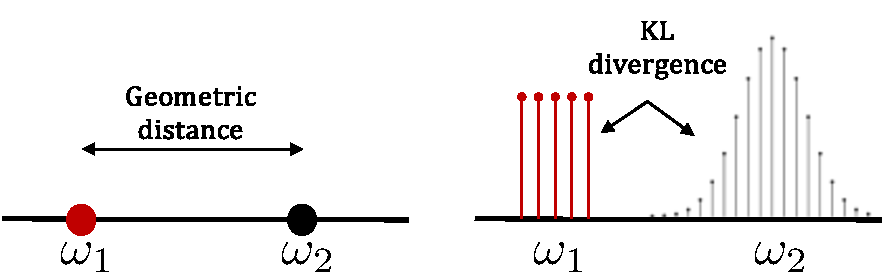
\includegraphics[width=\linewidth]{ill/shift_distance.pdf}
  \caption{The generalization of uniqueness.}
\end{figure}

We extend the preliminary version to handle the probabilistic case. 
We first systematically model uncertain property values in both continuous and discrete domains as continuous and discrete random variables, respectively.
Then, we consider the use of probability distributions, which are essential characteristics of uncertain property values, in the measuring similarity between uncertain property values. 
In this work, we use the well known Kullback-Leibler divergence to measure the distance between random variables with parameterized distributions. 

\begin{definition}
    \textbf{Uniqueness Score}
    Let $P$ be a property on the set of nodes $V$ of the input graph ,  
    let $d$ be the KL divergence function, 
    and let $\theta >0$  be a parameter. 
    Then the $\theta$-commonness of the property values $\omega$
    is $C_{\theta}(\omega)$ amounts to a weighted average over all other property values $\omega'$.    
     while the corresponding uniqueness is $U_{\theta}:= \frac{1}{C_{\theta}(\omega)}$. 
    \vspace{-5pt}
\end{definition} 
In the above definition, the weights decays exponentially as a function of the KL divergence among property values, 
and the parameter $\theta$ determines the decay rate. 
\begin{equation*}
  C_{\theta}(\omega) = \sum_{u \in V} \Phi_{\theta}(KL(\omega, P(v)))
\end{equation*}
In this work, we set $\theta=\sigma$ as the injected noise blurs the meta-distribution of property values. 
It should be noted that the commonness and uniqueness are meaningful only as relative measures. 
 
\textbf{Generalized Edge Relevance}~~
Alteration over a single edge would produce local structural change and send ripples through the rest of the graph. 
Even with the same amount of deviation, the incurred structural distortion varies on the topological role of the altered edge. 
Targets at the high utility, we should penalize edge modifications according to the incurred structural distortion.  
It naturally raises the need of measuring the relevance of edges in the probabilistic context. 

There are many potential ways to measure it. 
Importantly, the metric should be able to capture key properties of uncertain graphs.
Inspired by the importance of reliability, we measure the edge relevance of a given edge $e$ as the amount of structural distortion, measured by reliability discrepancy, caused by the unit noise subjects to the edge $e$, as follow. 
\begin{equation*}
  \begin{split}
    \mathcal{ERR}({e}) &= \frac{\Delta(\mathcal{G}+r_{e})}{|r_{e}|}  \\
                       &= \frac{\sum_{u,v} |R_{u,v}(\mathcal{G}+r_{e}) -R_{u,v}(\mathcal{G})|} {|r_{e}|}
  \end{split}
\end{equation*}

In the conventional case (deterministic graphs with edge addition and deletion $|r_{e}|=1$), it amounts to the connectivity distortion, measured by the deviation of \# of connected node pairs.  
In probabilistic graphs, $\mathcal{ERR}$ is used to generalize this concept by quantifying the stochastic impact of partial edge addition/deletion ($r_{e}$ lies in the contentious range) over the connectivity of all the possible worlds.
% It allows the estimation of structural distortion when $r_{e}$ lies in the contentious range. 
\begin{observation}
  Let $\mathcal{G}_{e}$, $\mathcal{G}_{\bar{e}}$ 
  denote two uncertain graphs that are identical to $\mathcal{G}$ with $p(e)=1$ and $p(e)=0$ respectively. 
  The reliability relevance of an edge $e$ is a constant and equivalent to 
  the following function. 
  \begin{equation}
    \mathcal{ERR}(e) = \sum_{u,v} R_{u,v}(\mathcal{G}_{e}) - \sum_{u,v} R_{u,v}(\mathcal{G}_{\bar{e}})
    \label{eq:err}
  \end{equation}
  Observe that, the edge relevance only depends on it topological location. 
  It amounts to the difference of the number of connected pairs between two neighbor uncertain graphs. 
\end{observation}

\textbf{Proof Sketch.}~~
According to the possible world semantics and factorization rule, we can see that   
\begin{equation*}
  R_{u,v} (\mathcal{G}) = p(e) \cdot R_{u,v}(\mathcal{G}_{e}) ~+~ \big[ 1-p(e) \big] \cdot R_{u,v} (\mathcal{G}_{\bar{e}})
\end{equation*}
Note that, the two-terminal reliability $R_{u,v}$ in $\mathcal{G}_{e}$ and $\mathcal{G}_{\bar{e}}$ are constants. 
Therefore, two-terminal reliability discrepancy introduced by the single deviation $r_{e}$ over the uncertain graph $\mathcal{G}$ is equivalent to 
\begin{equation*}
  \begin{split}
    \Delta_{u,v} (\mathcal{G}+r_{e}) ~&= r_{e} \cdot R_{u,v}(\mathcal{G}_{e}) - r_{e} \cdot R_{u,v} (\mathcal{G}_{\bar{e}})\\
    &= r_{e} \cdot ~\big[  R_{u,v}(\mathcal{G}_{e}) - R_{u,v} (\mathcal{G}_{\bar{e}})  \big]
  \end{split}
\end{equation*}
After aggregation and eliminating the factor $r_{e}$, we can see that the reliability relevance of an edge $e$ is equivalent to Equation~\ref{eq:err}. $\square$

Equation~\ref{eq:err} reminds us the basic concept of cut-edge. 
% What is the relationship between Equation~\ref{eq:err} and the conventional cut-edge definition? 
In a deterministic graph, a cut-edge is an edge of a graph whose deletion increase its number of connected components. 
We can see that the cut-edge is a binary version of $\mathcal{E}RR$.  
While $\mathcal{E}RR$ is a continuous function regarding the edge deviation $r_{e}$ and reliability discrepancy. 
$\mathcal{E}RR$ is not only relevant to connectivity discrepancy but also consider its scale.  

\textbf{Re-visiting the Computation Challenge}~~
\begin{figure}
    \subfigure[Iterative Evaluation]{\label{fig:itERR}
      \begin{minipage}[l]{0.46\columnwidth}
        \centering
        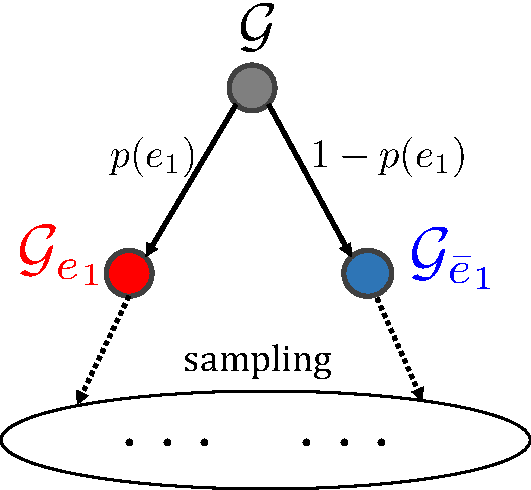
\includegraphics[height=2.7cm]{ill/iterativeERR.pdf}
      \end{minipage}
      }
    \subfigure[Memorized Evaluation]{\label{fig:groupERR}
      \begin{minipage}[l]{0.46\columnwidth}
        \centering
        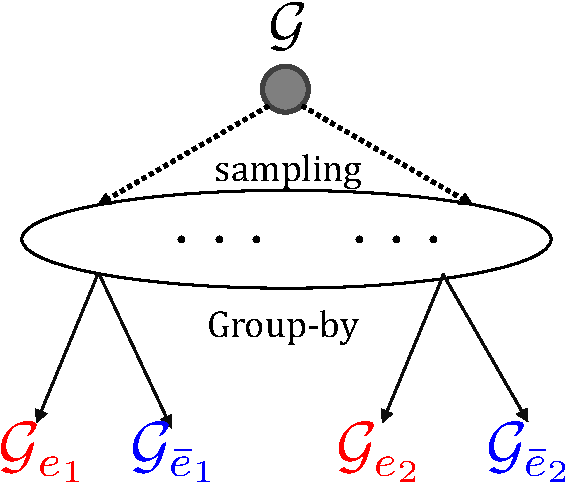
\includegraphics[height=2.7cm]{ill/groupERR.pdf}
      \end{minipage}
      }
    \vspace{-10pt}
    \caption{Sampling-based reliability detection}
    \vspace{-5pt}
    \label{fig:computationERR}
\end{figure} 
As shown in Equation~\ref{eq:err},  
the evaluation of $\mathcal{E}RR(e)$ involves a fundamental problem concerning uncertain graphs, which we call 
the Two-Terminal Reliability detection (TTR) problem. 
Since this problem is \#P-complete, we focus on efficiently and accurately approximate TTR.
The Monte-Carlo sampling method can be used to estimate the underlying reliability of an uncertain graph. 
Namely, we create a subset of possible worlds of the given uncertain graph with the use of edge sampling probabilities. 
Then, we take the average of the number of connected node pairs in the sampled worlds as an approximation. 
 
% The $\mathcal{E}RR$ evaluation over all the edges is not trivial. 
It is not trivial to evaluate $\mathcal{E}RR$ over all the edges. 
One option is to iterate sampling-based reliability computation over all the edges, 
as illustrated in Figure~\ref{fig:itERR}. 
It is straightforward to compute the connected components of a graph in linear time (regarding the numbers of the nodes and edges of the graph) using either breadth-first search or depth-first search.
For each edge, we need to perform the connected component detection for $N$ sampled graphs.
Thus, the overall time complexity is typically in the order of $\mathcal{O}( N |E|^{2})$.
Apparently, the iterative evaluation is inefficient when the uncertain input graph is massive.

Here, we present an efficient method with the time complexity in the order of $\mathcal{O}(N |E|)$.
As illustrated in Figure~\ref{fig:groupERR}, it memories the connected components detection result of samples. 
For evaluating the reliability relevance of one edge $e$, we group the sampled possible worlds according to the edge existence, 
then get the average value of $cc$ over each group as accurate approximation of $cc(\mathcal{G}_{e})$ and $cc(\mathcal{G}_{\bar{e}})$. 
Instead of sampling and evaluation from the scratch, we utilized the memorized results. 
The running time analysis roughly follows the analysis of the single-edge case.  
By this way, we bring the evaluation of edge reliability relevance to the realm.
\textbf{Edge Selection Boosted by Multi-heuristics}~~
To get the balance between anonymity and utility, we combined the generalized uniqueness metric $U$ and relevance $R$ metric by taking the ratio between them. 
We denote the combination as Balance Factor (BF) which is defined as follows:
\begin{equation*}
    BF(v)=\frac{U(v)}{R(v)}
\end{equation*}
For a give vertex $v$, $U(v)$ is the normalized uniqueness score of its property value among all the node in the original graph; $R(v)$ is the sum of reliability relevance of edges adjacent to the vertex. 
The higher value of BF represents the better trade-off between anonymity preserving and utility preserving. 
Our algorithm uses this heuristic to select and perturb the edge of uncertain graphs, as outlined in Algorithm 2. 




